\chapter{Introduction}
Cybersecurity has become a very important issue, thus, nowadays almost every system is built
with ICT (Information \& Communication Technologies).\\
\\
There are several ways in which the attack can create a damage:
\begin{itemize}
    \item \textbf{Financial Loss}: direct (e.g. fund transfer) or indirect (e.g. value of share or a fine by privacy authority).
    \item \textbf{Recovery Cost}: costs needed to take the system back to normal operations and/or to improve its security features;
        
    \item \textbf{Productivity loss:} because the processes being stopped or delayed.
    \item \textbf{reputation damage:} if you are a company and yo are being attacked it's difficult to regain trust.
\end{itemize}
Another a big problem nowadays is the complexity of the scenario \textit{Information Communication Technology} (ICT):
\begin{itemize}
    \item  \textbf{"Personal" devices:} 
    \begin{itemize}
        \item \underline{desktop, laptop, tablet, smartphone, ...}
        \item \underline{smart TV, fridge, car, ...}
    \end{itemize}
    
    \item \textbf{Communication networks:}
    \begin{itemize}
        \item \underline{data-only network}: In the past we had two independent networks, the telephone network and the data network. But nowadays is no more like that, the  telephone is going on data, so if the data network not working, the analogic network not working.
        \item \underline{Wired and wireless networks} 
        \item \underline{Mobility} (mobility means trustability, I can detect where you are allocated)  
    \end{itemize}
    \item \textbf{Distribute devices}: company are trying to give out computer and networks, but it's means that you are not controlling your computer (outsourcing, hosting, farming, cloud, IoT).
    \item \textbf{Programming become increasingly complex}: stratification, framework, libraries etc... 
\end{itemize}
\begin{quotebox-yellow}{First Axiom of Engineering}
    The more complex is, the more difficult its correctness verification will be (implementation, management, operation).
\end{quotebox-yellow}
\noindent
\textbf{Example:} the number of bugs in a program is proportional to its number of lines of code. 
\newline
\\ \textcolor{red}{\textbf{N.B.}} The complexity of the current information systems is in favour of the attackers that find attack paths increasingly ingenious and unforeseen by the defenders.

\newpage
\section{Risk estimation}
If you want to create some kind of protection, the first step is \textbf{to understand the risks}. Analyzing a system and its service in search of risk means finding the:
    \\
    \\
    \begin{minipage}{0.6\textwidth}
    %	\vspace{-0.5cm}
    \begin{itemize}
        \item \textbf{Assets}: set of ICT resources, data, people and locations needed for an IT service which needed to be protected.
        \item The \textbf{events}, represents the potential issues or incident that can affect the assets. Events are linked to two key concepts:
        \begin{itemize}
            \item \underline{Vulnerabilities}: intrinsic weakness of an asset (e.g.login; sensible to flooding).
            \item \underline{Threats}: possible deliberate action/accidental event that can produce the loss of security property by exploiting a vulnerability. (It depends upon the specific environment and/or operating conditions)
        \end{itemize} 
    \end{itemize}
    \end{minipage} 
    \hspace{0.2cm}
    \begin{minipage}{0.4\textwidth}
        \vspace{-1cm}
        \centering
        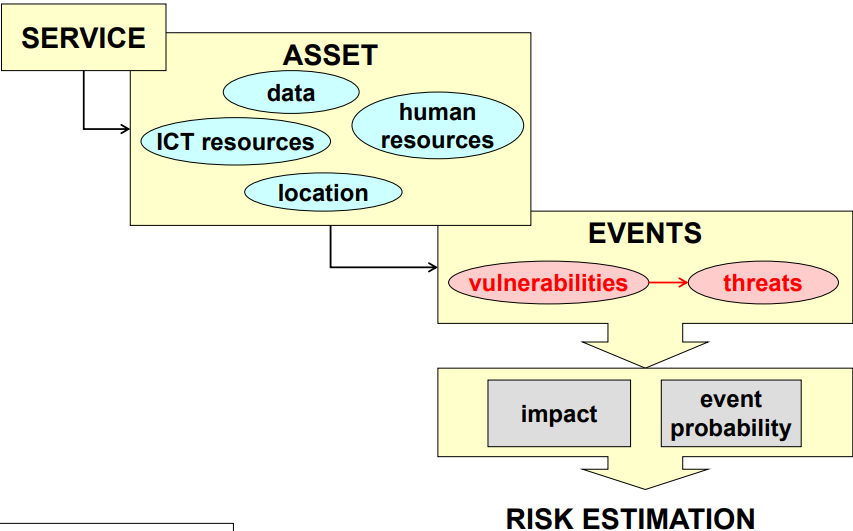
\includegraphics[width=1\textwidth]{/home/lorenzo/Notes/Information System Security/images/image copy 3.png}
    \end{minipage}
    \begin{quotebox-grey}{What is the correct time to think about security when we develop a system?}
        During the development of a system, security \textbf{must} be taken into account at every step of its lifecycle. 
        \\
            \begin{center}
                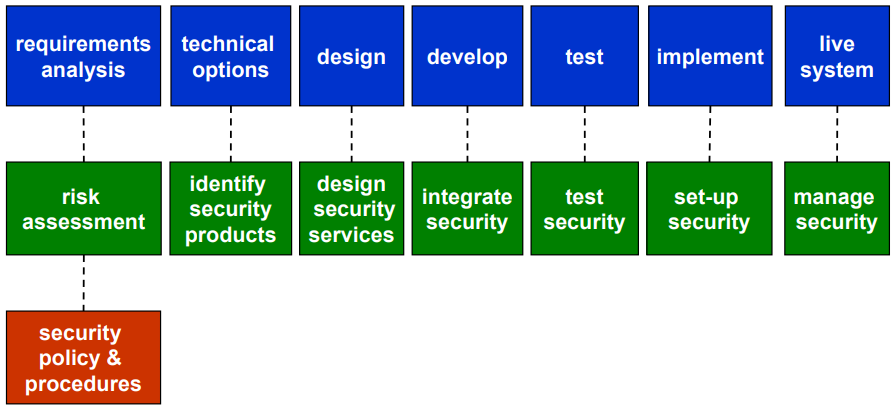
\includegraphics[width=0.5\textwidth]{/home/lorenzo/Notes/Information System Security/images/image copy 6.png}
            \end{center}
    \end{quotebox-grey}
    
    \noindent
    \\
    \begin{minipage}{0.6\textwidth}
        %	\vspace{-0.5cm}
        After the identification of the risk, we need to prioritize them keeping into account not only the impact but also the available time and budget. 
        A risk assessment matrix (or risk heat map) may be useful. On the X-axis, we have the \textbf{probability} while on the Y-axis, we have the \textbf{impact}. Both of them are represented by a numerical score and each cell in the matrix is calculated by multiplying the impact by the probability:
    \end{minipage} 
    \hspace{0.2cm}
    \begin{minipage}{0.4\textwidth}
            \centering
            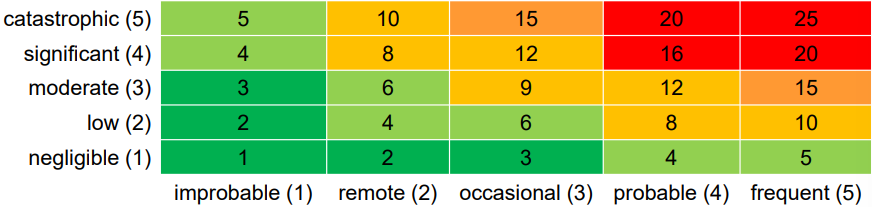
\includegraphics[width=\textwidth]{/home/lorenzo/Notes/Information System Security/images/image copy 4.png}
    \end{minipage}

\section{Risk Management}
\begin{minipage}{0.5\textwidth}
	\vspace{-1.0cm}
After identifying the risks, we had to select possible countermeasures and implement them. Following this, we need to take the exam, which in real life is \textbf{Audit}: an independent person/company that checks if the countermeasures are effective.\\
\\
The solution in this graph is represented by the \textbf{Security control},
which is a element that you put in place to create some security
features, to match the security requirement. (For example, the
seatbelt is a security control for a car).
\end{minipage} 
\hspace{0.3cm}
\begin{minipage}{0.5\textwidth}
    
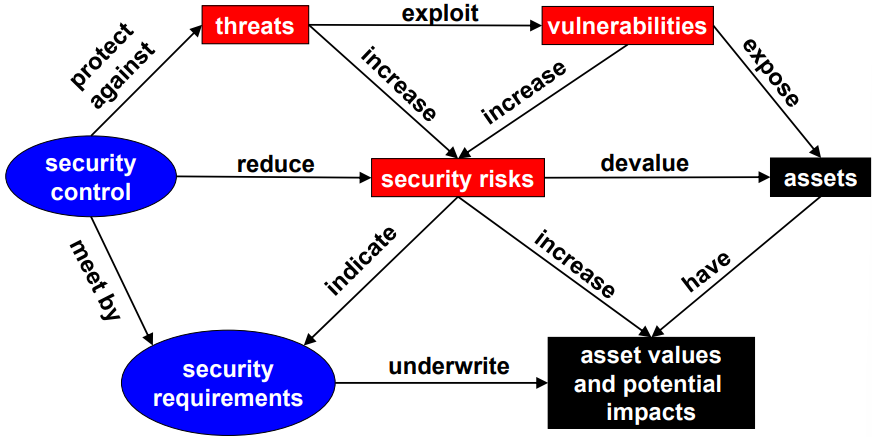
\includegraphics[width=1\textwidth]{/home/lorenzo/Notes/Information System Security/images/image copy 7.png}
\end{minipage}

\begin{quotebox-grey}{Some terminology}
    \begin{itemize}
        \item \textbf{Incident}: a security event that compromises the integrity, confidentiality, or availability of an information asset.
        \item  \textbf{(data) breach}: an incident that results in the disclosure or potential exposure of data. 
        \item \textbf{(data) disclosure}: a breach for which it was confirmed that data was actually disclosed (not just exposed) to an unauthorized party.
    \end{itemize}
\end{quotebox-grey}



\section{Window of exposure}

\begin{figure}[H]
    \centering
    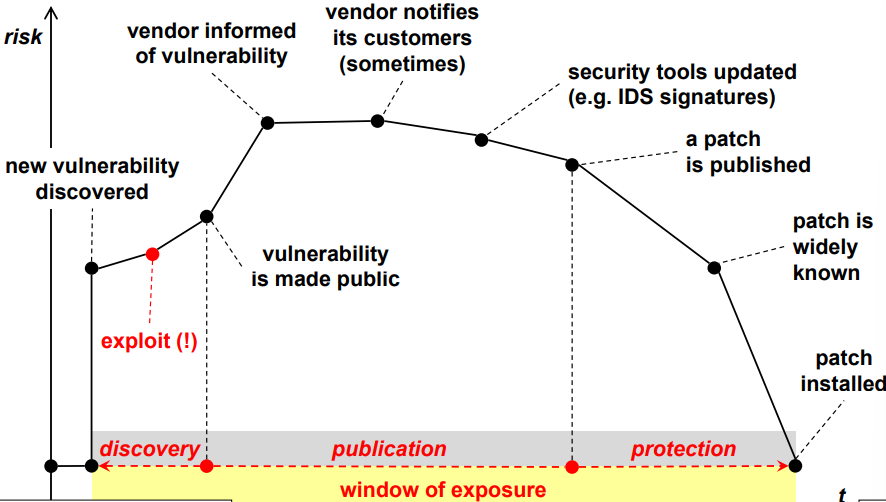
\includegraphics[width=0.5\textwidth]{/home/lorenzo/Notes/Information System Security/images/image copy 8.png}
\end{figure}
\begin{enumerate}
    \item \textbf{New vulnerability discovered}: this is the point where a vulnerability in a system is first discovered by a researcher or an attacker. The risk start to increase as this vulnerability can be exploited if it becomes known to malicious actors.
    \item \textbf{Vulnerability is made public}: the vulnerability is disclosed publicly. This increases the risk further because now the attackers may attempt to exploit it. 
    \item \textbf{Vendor informed of vulnerability}: the vulnerability is reported to the vendor. At this point, the vendor can start working on a fix or patch.
    \item \textbf{Vendor notifies its costumers (sometimes)}: Sometimes the vendor informs its customers about the vulnerability and the steps they can take to protect their systems.
    \item \textbf{Security tools updated}: Security tools like Intrusion Detection Systems (IDS) or antivirus programs are updated to detect and mitigate attacks.
    \item \textbf{A patch is published}: The vendor releases a patch or software update that fixes the vulnerability.
    \item \textbf{Patch is widely known}: The patch becomes well-known and more organizations become aware of it. The risk continues to decrease as more systems apply the patch.
    \item \textbf{Patch installed}: When the patch is finally installed across systems, the vulnerability is completely resolved, and the risk drops to nearly zero. 
\end{enumerate}

\section{Cyber threats}
\begin{minipage}{0.7\textwidth}
%	\vspace{-0.5cm}
\textbf{Cyber Threat} are composed by 3 main components:
\begin{itemize}
    \item \textbf{Threat actors}: they usually follow a set of \textbf{MICE} motivations:
    \begin{itemize}
        \item \textbf{M}oney: direct transfer, blackmail, ... or indirect (etc. data reselling).
        \item \textbf{I}deology: political, religious, hacktivism,...
        \item \textbf{C}ompromise: individuals with no choice due to blackmail or threat against their families or themselves.
        \item \textbf{E}go: bragging around and positive reputation.

    \end{itemize}
    \item \textbf{Attack vectors} (vulnerabilities and context)
    \item \textbf{vulnerable targets} (value for owner and attacker)
\end{itemize} 
\end{minipage} 
\hspace{0.3cm}
\begin{minipage}{0.4\textwidth}
    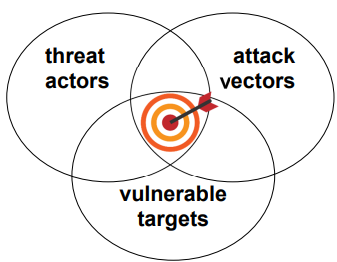
\includegraphics[width=0.8\textwidth]{/home/lorenzo/Notes/Information System Security/images/image copy 9.png}
\end{minipage}
\\
\\
\noindent
\textcolor{red}{\textbf{N.B.}} To successfully execute a cyber threat, there must be an intersection of all three elements.


\section{Standardization bodies}
\begin{figure}[H]
    \centering
    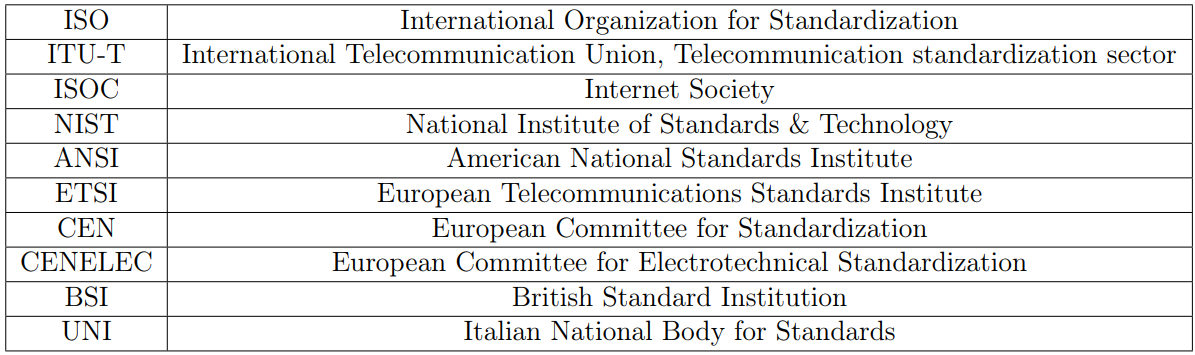
\includegraphics[width=0.8\textwidth]{/home/lorenzo/Notes/Information System Security/images/Screenshot from 2024-12-27 10-23-19.png}
\end{figure}

\section{Security}
\begin{quotebox-yellow}{}
\textbf{Security} is \textbf{not} a product, but a \textbf{process} that recognizes the inherit insecurity in the products.\\
Flaws, vulnerabilities and risks are \textbf{inevitable} \(\rightarrow \) we \textbf{must} try to reduce the risk of exposure regardless of the products and patches.
\end{quotebox-yellow}
\noindent
In order to do so, security needs to follow a series of core \textbf{principles}:
\begin{itemize}
    \item \textbf{Security in depth}: this principle promotes for implementing multiple layers of security controls throughout an information system. The idea is that if one layer fails, additional layers can still provide protection. 
    \item \textbf{Security by design}: means integrating security measures into the design and development process of systems and applications from the outset, rather than as an afterthought.
    \item \textbf{Security by default}: refers to configuring systems to a secure state out of the box, without requiring additional user intervention.
    \item \textbf{Least privilege}: stipulates that users and systems should be granted the minimum level of access necessary to perform their functions.
    \item \textbf{Need-to-know}: this principle  principle restricts access to sensitive information to only those individuals who require it to perform their job functions.
\end{itemize}

\begin{quotebox-grey}{C.I.A}
    \begin{minipage}{0.7\textwidth}
    %	\vspace{-0.5cm}
        The most important security principles can be summarized with the acronym \textbf{C.I.A.}:
        \begin{itemize}
        \item \textbf{Confidentiality}: ensuring that sensitive information is accessed only by authorized individuals.
        \item \textbf{Integrity}: ensuring the accuracy, consistency, and trustworthiness of data over its life cycle.
        \item \textbf{Availability}: ensuring that information and resources are available to authorized users when needed.    
    \end{itemize}
    \end{minipage} 
    \hspace{0.3cm}
    \begin{minipage}{0.3\textwidth}
        \centering
        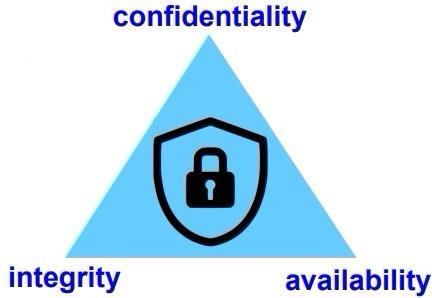
\includegraphics[width=0.8\textwidth]{/home/lorenzo/Notes/Information System Security/images/image copy 5.png}
    \end{minipage}

\end{quotebox-grey}
\subsection{Other security properties}
\begin{itemize}
    \item \textbf{Authenticity}:is the property of being genuine and able to verify that you are trusted. Authenticity can be verified in two ways:
    \begin{itemize}
            \item \underline{Simple Authentication}: only one party in the communication (usually the user) is required to prove their identity to the other party (usually the system or server).
            \item \underline{Mutual Authentication}: both parties involved in the communication must prove their identities to each other. 
    \end{itemize} 
    \item \textbf{Data Authentication}: is the process of verifying that the data received or accessed is genuine and has not been altered during transmission or storage.
    \item \textbf{Origin Authentication}: is the process of verifying the identity of the source or sender of the data, ensuring that the data actually comes from a legitimate or intended sender.
    \item \textbf{Authorization}: is a critical concept that defines what an authenticated user or system is allowed to do after they are successfully identified.
    \item \textbf{Non-repudiation}: Non-repudiation provides a formal proof that is legally acceptable, ensuring that a person or system cannot deny having created, sent, or received a particular message or data.
    \item \textbf{Accountability/Traceability}: is the security goals that generates the requirement for actions of an entity to be traced \textbf{uniquely} to that entity.
\end{itemize}
\newpage
\section{Data protection}
For each security property, consider always the three cases of data protection:
\begin{enumerate}
    \item \textbf{"data in transit"} : when data are transmitted over a communication channel. 
    \item \textbf{"data at rest"}: when data are stored in a memory device.
    \item \textbf{"data at work"}: when data are in RAM for use by a process.
\end{enumerate}
\begin{quotebox}[colframe=blue!10!white, colback=blue!5!white]{Where is the enemy?}
    One of the first question when we want to create some kind of protection is where is the enemy is located:
    \begin{itemize}
        \item \textbf{Outside our organization}: in this case the kind of defence is called boundary/perimeter defence (firewall).
        \item \textbf{Outside our organization, with the exception of our partners}: in this case we will implement extranet protection (VPN). [Extranet: when you network is extended to connect to other networks].
        \item \textbf{Inside our organization}: we should protect the Local Area Network, this is much more difficult because the LAN are built to cooperate. 
        \item \textbf{Everywhere}: having a defence which is based on the position today become meaningless.    
    \end{itemize}
\end{quotebox}
Nowadays having a defence based on the position is meaningless. The alternative is to think that the attackers are \textbf{everywhere}. That is a new modern architecture, called \textbf{ZTA (Zero Trust Architecture)}. This allows the system to be completely protected by various form of attacks, both \textbf{passive} (can \textbf{only read} the data/traffic) and \textbf{active} (can \textbf{read} but also \textbf{modify},\textbf{delete} or \textbf{create} data/traffic). We can also classify attackers based on their position:
\begin{itemize}
    \item \underline{MITM (Man-In-The-Middle)}: sitting between the two peers A and B.
    \item \underline{MATE (Man-At-The-End)}: inside one peer.
    \item \underline{MITB (Man-In-The-Browser)}: inside a component of a peer (typically, the web browser).   
\end{itemize}

\section{Technological Attacks}
The networks are (almost) always insecure, since most of them use wireless connections \(\rightarrow \) communication via broadcast. Moreover, most networks have access to geographical connections are that not made through end-to-end dedicated lines, but through shared lines
and third-party routers. Weak user authN, lack of server side authN and software bugs are also
contributing factors to the successfulness and likelihood of an attack.
Technological Attacks can be divided in various classes: 
\begin{itemize}
    \item \underline{\textbf{IP spoofing (masquerading)}}: IP spoofing is when someone uses the address of another host, to take its place as a client (and hide its own actions) or as a server. The spoofing usually happens at \textbf{Layer 3}, which is the \textbf{IP address}. IP spoofing can also happens at \textbf{Layer 2}. A better name would be \textbf{source address spoofing} because this kind of attack, as we said before, it can also happens at Layer 2.\\
    \\
    \textcolor{green}{\textbf{Countermeasures}}: Avoid address-based authentication.
    \item \underline{\textbf{Packet sniffing (eavesdropping)}}: With a packet sniffing attack I can read packets that are not addressed to me, but
    to another network node. If you are on a broadcast network, this is very easy, you
    just need to put my network card in promiscuous mode (which accept all packet even if the address doesn’t match with the destination packet).\\
    \\
    \textcolor{green}{\textbf{Countermeasures}}:
    \begin{itemize}
        \item \textbf{Don't use broadcast networks}, but it's difficult because must of the networks are broadcast.  
        \item \textbf{Encryption of packet payload} (No the header because it contains the destination).
    \end{itemize}
    \item \underline{\textbf{Denial-of-service (distributed DoS)}}: Dos is a attack against availability, he keep a host busy so that it can't provide its services.\\
    \\
    \textcolor{green}{\textbf{Countermeasures}}: We don’t have any countermeasures. Monitoring and over-sizing (in other words,making the system bigger than is needed) can mitigate the effects.
    \newpage
    \item \underline{\textbf{Distributed denial-of-service (DDOS)}}:
    \\
    \begin{minipage}{0.6\textwidth}
    \vspace{0.3cm}
    Attacker can spread the DoS software on many nodes (called daemons, zombies or malbots) to create a Botnet. Daemons are controlled remotely by a master node through encrypted channels (e.g. UDP packets contained inside the payload of ICMP Echo Requests),this distribution multiplies the effect of the DoS attacks by a factor equal to the number of daemons. \\\textbf{DDoS} attacks’ effectiveness can be improved further in two ways:
    \begin{itemize}
        \item \textbf{Reflectors}: the attacker can hide his tracks by using a legitimate third-party server.
        \item \textbf{Amplification Factor N:1}: the attacker looks for a reflector server that amplifies the attack scale by a factor of N (depends on the used protocol).
    \end{itemize}

    \end{minipage} 
    \hspace{0.2cm}
    \begin{minipage}{0.4\textwidth}
        \centering
        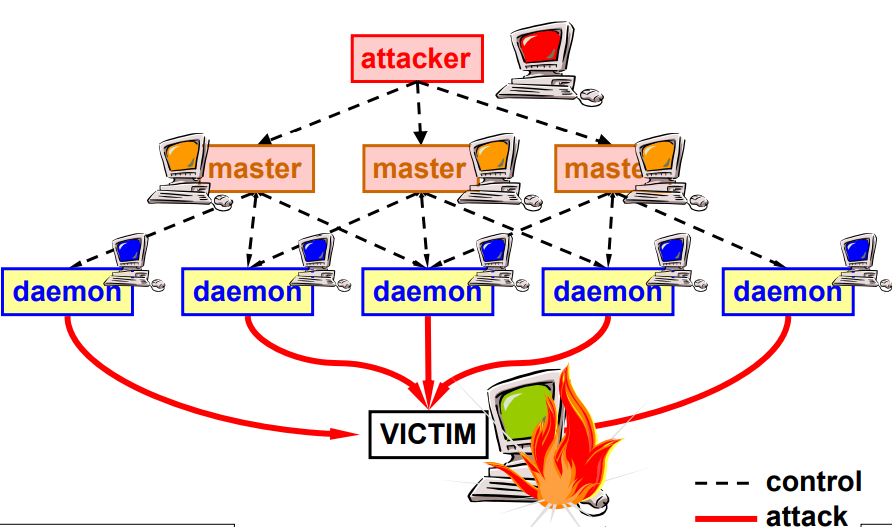
\includegraphics[width=0.8\textwidth]{/home/lorenzo/Notes/Information System Security/images/image copy 10.png}
    \end{minipage}
\item \underline{\textbf{Shadow/fake server}}: The attacker manages to show itself to the victims as a service provider server without having the right to do so. To achieve this, the attacker must sniff the requests and spoof (elaborate) responses faster than the real server (e.g. can be achieved with a superior computer or via DDoS attack) or it can manipulate the routing/DNS tables. The objective of the attack is to gain knowledge of the victim’s data.\\ 
\\  
\textcolor{green}{\textbf{Countermeasures}}:  possible countermeasure is to guarantee the server authentication.
\item \underline{\textbf{Trojan}}: A Trojan is a program that contains a dangerous payload. Typically that’s done because network channels are more protected but user terminals are less protected
(e.g. Smartphone, IoT, "ignorant" users [also people who want to save money]).\\ Trojan are usually difficult to remove as they use \textbf{stealth techniques} to stay undetected.
\item \underline{\textbf{Software bug}}: In general even the best software contains bugs that can be exploited by attackers. The easiest way to exploit the bugs is DoS.
\item \underline{\textbf{Malware}}: Malware is a generic term that refers to all types of malicious software. It's specifically designed to harm, exploit, or otherwise compromise the security of computer systems, networks, or devices. There are many types of malware:
\begin{itemize}
    \item \textbf{Virus} is a program or application that damages the target and replicates itself. The virus has not the ability to propagate by itself, it's propagated by humans (involuntarily).
    \item \textbf{Worm} is typically a malware that does not create damage directly, instead he damages the target by replicating itself, there by saturating the resources. It's capable to do a automatic propagation.
    \item \textbf{Trojan}: malware vector.
    \item \textbf{Backdoor}: it's a hidden entry point in your system. In some cases the backdoor is inserted by the police/army to foot inside an organization.
    \item \textbf{Rootkit:} it's a software that it's been downloaded in your system which is providing privileged access. It remains hidden (by modifying programs, libraries, drivers, kernel modules, or hypervisors) and operates stealthily.
    \item \textbf{PUA (Potentially Unwanted Applications)}: These are software programs that may not be malicious in nature, but they can negatively impact your system's performance or privacy. PUAs are often bundled with legitimate software or downloaded inadvertently by users.
\end{itemize}
\noindent
\textcolor{green}{\textbf{Countermeasures}}: \begin{itemize}
    \item \textbf{User awareness}
    \item \textbf{Correct configuration/Secure software}
    \item \textbf{Install antivirus} (and keep updated!)
\end{itemize}
\begin{quotebox-grey}{Ransomware}
    It’s the most frequent kind of \textbf{malware} distributed nowadays. A ransowmware is a malware oriented to get a ransom (a "ransom" is a sum of money demanded for the release of someone who has been kidnapped or captured). Typically he arrived
    on your device and encrypt your PC with a key that you don’t know, so you will not be able to read your file. You need to pay if you want your data back.\\ 
    \textcolor{green}{\textbf{Countermeasures}}: A possible countermeasure consists of doing regular backups, the backup must be offline; otherwise, it can be attacked as well. However we need to pay attention to how old the backup is, because nowadays there is \textbf{silent ransomware}, this type of ransomware doesn't block your PC immediately; it encrypts your system.
\end{quotebox-grey}
\end{itemize}

\begin{quotebox}[colframe=blue!10!white, colback=blue!5!white]{Cyber Theft Ring}
\begin{minipage}{0.5\textwidth}
%	\vspace{-0.5cm}
The cyber theft ring is a criminal organization involved in stealing money through online means. 
\begin{itemize}
    \item \textbf{Malware Coders}: These individuals create malicious software (malware) that is sold on the black market. This software is used to attack victims' computers and steal their personal information, including banking credentials.
    \item \textbf{Malware Exploiters}: These individuals purchase malware from coders and use it to launch attacks on victims.
    \item \textbf{Money Mules}: These are individuals recruited to launder stolen funds. They are paid a percentage of the stolen money for their services. Money mules often transfer funds between different accounts to make it difficult for authorities to trace the money's origin.   
    \item \textbf{Victims}: : The targets of cyber theft can include individuals, businesses, and financial institutions.
\end{itemize} 
\end{minipage} 
\hspace{0.2cm}
\begin{minipage}{0.4\textwidth}
    \centering
    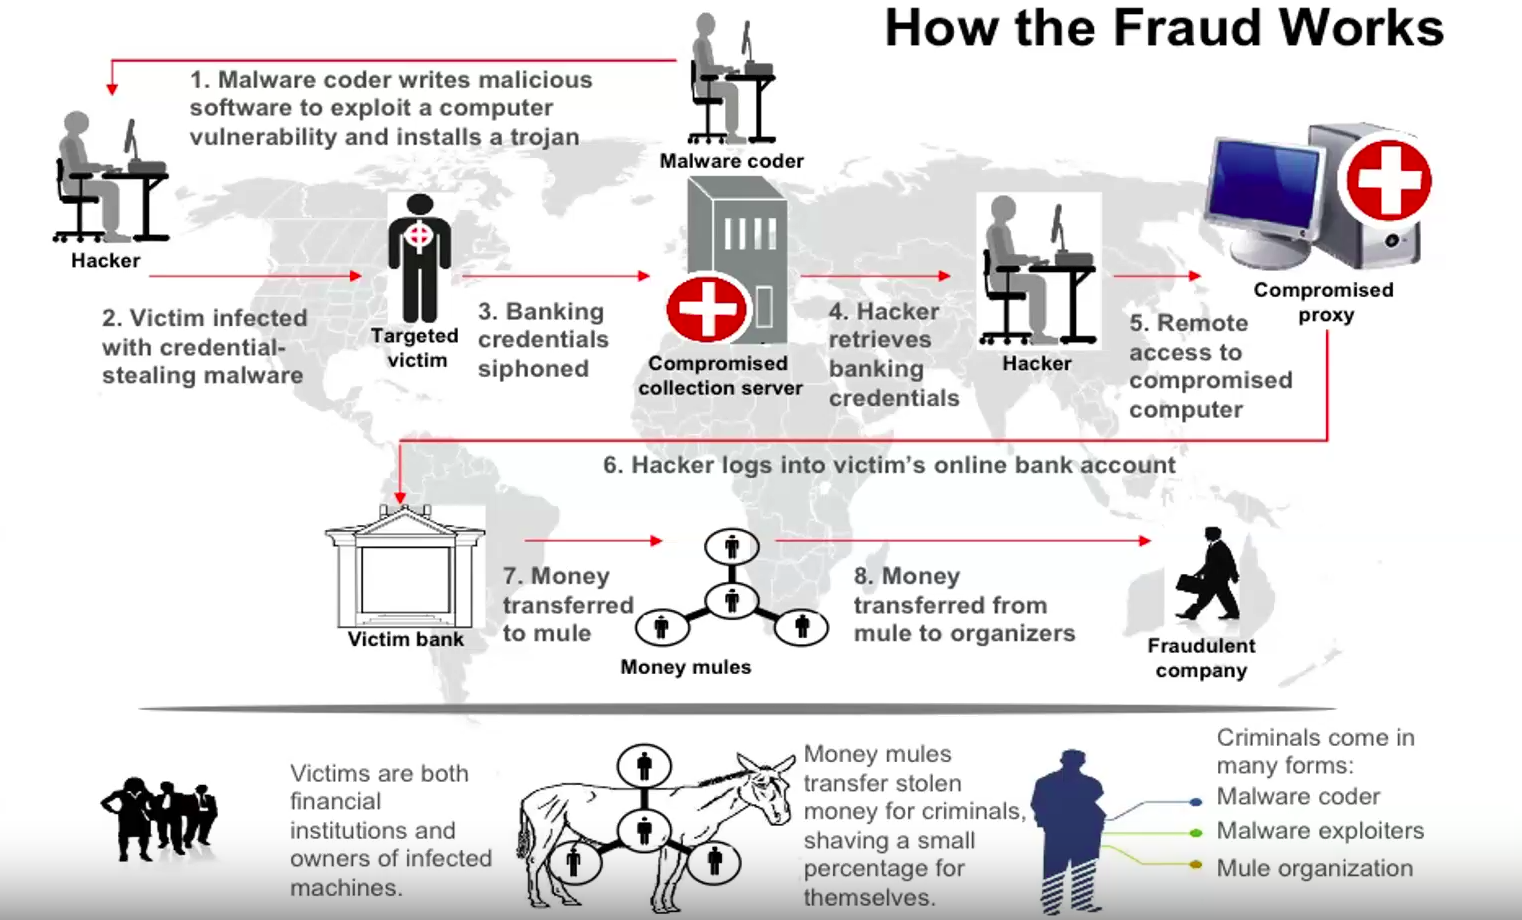
\includegraphics[width=1.2\textwidth]{/home/lorenzo/Notes/Information System Security/images/image copy 11.png}
\end{minipage}
\end{quotebox}

\section{Technology and human beings}
\begin{minipage}{0.6\textwidth}
	\vspace{-0.5cm}
No matter how strong the technological defenses are, \textbf{human error remains a major vulnerability in cybersecurity}. Even with the best tools, human mistakes can undermine security efforts. The non technological problems are various:
\begin{itemize}
    \item People don't understand the problem
    \item Mistake of human beings (especially when overloaded, stressed, ...).
    \item Complex interfaces/architectures can mislead the user and originate erroneous behaviours. 
    \item Performance decrease due to the application of security measures.
\end{itemize}
\end{minipage} 
\hspace{0.5cm}
\begin{minipage}{0.4\textwidth}
    \centering
    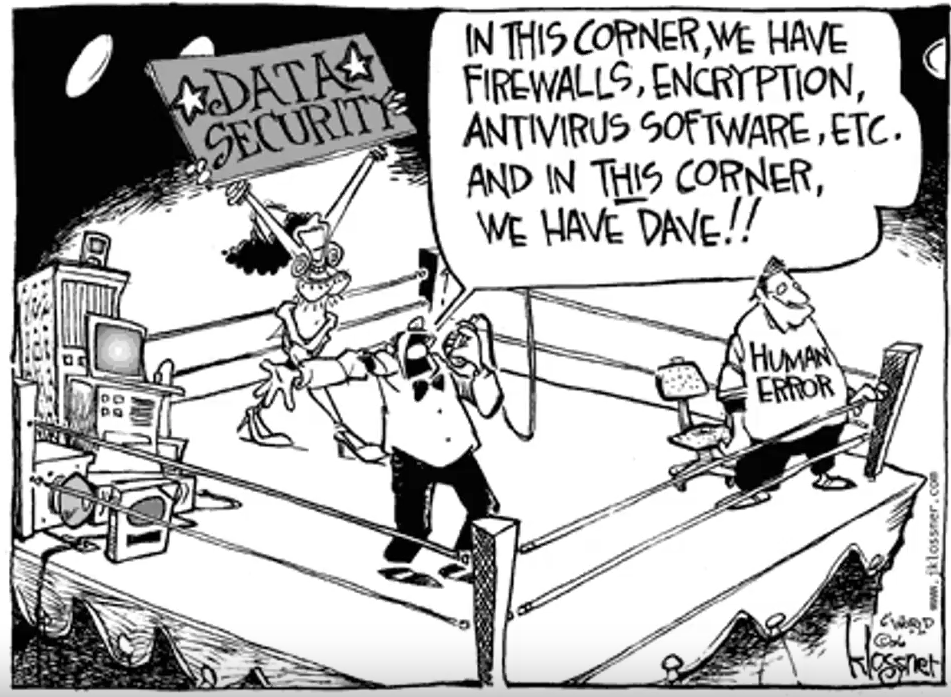
\includegraphics[width=\textwidth]{/home/lorenzo/Notes/Information System Security/images/image copy 12.png}
\end{minipage}
\\
\\
\noindent{\color{gray!50}\rule{\textwidth}{0.5pt}}













 